%%%%%%%%%%%%%%%%%%%%%%%%%%%%%%%%%%%%%%%%%%%%%%%%%%%%%%%%%%%%%%%%%%%%%%
%%  Copyright by Wenliang Du.                                       %%
%%  This work is licensed under the Creative Commons                %%
%%  Attribution-NonCommercial-ShareAlike 4.0 International License. %%
%%  To view a copy of this license, visit                           %%
%%  http://creativecommons.org/licenses/by-nc-sa/4.0/.              %%
%%%%%%%%%%%%%%%%%%%%%%%%%%%%%%%%%%%%%%%%%%%%%%%%%%%%%%%%%%%%%%%%%%%%%%

\newcommand{\commonfolder}{../../common-files}
\documentclass[11pt]{article}

\usepackage[most]{tcolorbox}
\usepackage{times}
\usepackage{epsf}
\usepackage{epsfig}
\usepackage{amsmath, alltt, amssymb, xspace}
\usepackage{wrapfig}
\usepackage{fancyhdr}
\usepackage{url}
\usepackage{verbatim}
\usepackage{fancyvrb}
\usepackage{adjustbox}
\usepackage{listings}
\usepackage{color}
\usepackage{subfigure}
\usepackage{cite}
\usepackage{sidecap}
\usepackage{pifont}
\usepackage{mdframed}
\usepackage{textcomp}
\usepackage{enumitem}
\usepackage{hyperref}


% Horizontal alignment
\topmargin      -0.50in  % distance to headers
\oddsidemargin  0.0in
\evensidemargin 0.0in
\textwidth      6.5in
\textheight     8.9in 

\newcommand{\todo}[1]{
\vspace{0.1in}
\fbox{\parbox{6in}{TODO: #1}}
\vspace{0.1in}
}


\newcommand{\unix}{{\tt Unix}\xspace}
\newcommand{\linux}{{\tt Linux}\xspace}
\newcommand{\minix}{{\tt Minix}\xspace}
\newcommand{\ubuntu}{{\tt Ubuntu}\xspace}
\newcommand{\setuid}{{\tt Set-UID}\xspace}
\newcommand{\openssl} {\texttt{openssl}}


\pagestyle{fancy}
\lhead{\bfseries SEED Labs}
\chead{}
\rhead{\small \thepage}
\lfoot{}
\cfoot{}
\rfoot{}


\definecolor{dkgreen}{rgb}{0,0.6,0}
\definecolor{gray}{rgb}{0.5,0.5,0.5}
\definecolor{mauve}{rgb}{0.58,0,0.82}
\definecolor{lightgray}{gray}{0.90}


\lstset{%
  frame=none,
  language=,
  backgroundcolor=\color{lightgray},
  aboveskip=3mm,
  belowskip=3mm,
  showstringspaces=false,
%  columns=flexible,
  basicstyle={\small\ttfamily},
  numbers=none,
  numberstyle=\tiny\color{gray},
  keywordstyle=\color{blue},
  commentstyle=\color{dkgreen},
  stringstyle=\color{mauve},
  breaklines=true,
  breakatwhitespace=true,
  tabsize=3,
  columns=fullflexible,
  keepspaces=true,
  escapeinside={(*@}{@*)}
}

\newcommand{\newnote}[1]{
\vspace{0.1in}
\noindent
\fbox{\parbox{1.0\textwidth}{\textbf{Note:} #1}}
%\vspace{0.1in}
}


%% Submission
\newcommand{\seedsubmission}{
Debe enviar un informe de laboratorio detallado, con capturas de pantalla, para describir lo que ha hecho y lo que ha observado.
También debe proporcionar una explicación a las observaciones que sean interesantes o sorprendentes.
Enumere también los fragmentos de código más importantes seguidos de una explicación. No recibirán créditos aquellos fragmentos de códigos que no sean explicados.}

%% Book
\newcommand{\seedbook}{\textit{Computer \& Internet Security: A Hands-on Approach}, 2nd
Edition, by Wenliang Du. Para más detalles \url{https://www.handsonsecurity.net}.\xspace}

%% Videos
\newcommand{\seedisvideo}{\textit{Internet Security: A Hands-on Approach},
by Wenliang Du. Para más detalles \url{https://www.handsonsecurity.net/video.html}.\xspace}

\newcommand{\seedcsvideo}{\textit{Computer Security: A Hands-on Approach},
by Wenliang Du. Para más detalles \url{https://www.handsonsecurity.net/video.html}.\xspace}

%% Lab Environment
\newcommand{\seedenvironment}{Este laboratorio ha sido testeado en nuestra imagen pre-compilada de una VM con Ubuntu 16.04, que puede ser descargada del sitio oficial de SEED.\xspace}

\newcommand{\seedenvironmentA}{Este laboratorio ha sido testeado en nuestra imagen pre-compilada de una VM con Ubuntu 16.04, que puede ser descargada del sitio oficial de SEED.\xspace}

\newcommand{\seedenvironmentB}{Este laboratorio ha sido testeado en nuestra imagen pre-compilada de una VM con Ubuntu 20.04, que puede ser descargada del sitio oficial de SEED .\xspace}

\newcommand{\seedenvironmentC}{Este laboratorio ha sido testeado en nuestra imagen pre-compilada de una VM con Ubuntu 20.04, que puede ser descargada del sitio oficial de SEED. Sin embargo, la mayoría de nuestros laboratorios pueden ser realizados en la nube para esto Ud. puede leer nuestra guía que explica como crear una VM de SEED en la nube.\xspace}

\newcommand{\seedenvironmentAB}{
Este laboratorio ha sido testeado en nuestras imagenes pre-compiladas de una VM con Ubuntu 16.04 y otra con Ubuntu 20.04, que pueden ser descargadas del sitio oficial de SEED.\xspace}

\newcommand{\nodependency}{Dado que utilizamos contenedores para configurar el entorno de laboratorio, este laboratorio no depende estrictamente de la VM de SEED. Puede hacer este laboratorio utilizando otras máquinas virtuales, máquinas físicas o máquinas virtuales en la nube.\xspace}

\newcommand{\adddns}{You do need to add the required IP address mapping to
the \texttt{/etc/hosts} file.\xspace}






\newcommand{\seedlabcopyright}[1]{
\vspace{0.1in}
\fbox{\parbox{6in}{\small Copyright \copyright\ {#1}\ \ by Wenliang Du.\\
      Este trabajo se encuentra bajo licencia Creative Commons.
       Attribution-NonCommercial-ShareAlike 4.0 International License.
       Si ud. remezcla, transforma y construye a partir de este material,
       Este aviso de derechos de autor debe dejarse intacto o reproducirse de una manera que sea razonable para el medio en el que se vuelve a publicar el trabajo.
       }}
\vspace{0.1in}
}






\newcommand{\telnet} {\texttt{telnet}\xspace}
\newcommand{\iptables}{\texttt{iptables}\xspace}
\newcommand{\netfilter}{\texttt{netfilter}\xspace}
\newcommand{\Netfilter}{\texttt{Netfilter}\xspace}

\newcommand{\firewallFigs}{./Figs}
\lhead{\bfseries SEED Labs -- Laboratorio Exploratorio de Firewall}

\newcommand{\pointleft}[1]{\reflectbox{\ding{217}} \textbf{\texttt{#1}}}

\begin{document}

\begin{center}
{\LARGE Laboratorio Exploratorio de Firewall}
\end{center}

\seedlabcopyright{2006 - 2021}



% *******************************************
% SECTION
% ******************************************* 
\section{Descripción}

El objetivo de este laboratorio es separado en dos partes: aprender como funciona un firewall y configurar un firewall simple para una red. Los estudiantes primero implementarán un firewall simple para filtrar paquetes, este firewall se encargará de inspeccionar estos paquetes y decidirá cuando rechazarlos o cuando dejarlos pasar, todo esto basado en una serie de reglas del firewall.
Usando esta implementación los estudiantes podrán conocer las ideas básicas del funcionamiento de un firewall.

En la actualidad, los sistemas linux tienen integrado un firewall, basado en \texttt{netfilter}. Este firewall se llama \iptables. 
Los estudiantes tendrán disponible una topología de red simple, y serán los encargados de configurar reglas de firewall para proteger esta red.
Los estudiantes podrán experimentar diferentes tipos de usos con \iptables. 

Este laboratorio cubre los siguientes tópicos:


\begin{itemize}[noitemsep]
\item Firewall
\item Netfilter
\item Módulo del Kernel (LKM)
\item Usando \iptables para reglas de firewall
\item Varios usos de \iptables
\end{itemize}


\paragraph{Lecturas y Videos.}
Para una cobertura más detallada sobre firewalls puede consultar:

\begin{itemize}
\item Capítulo 17 del libro de SEED, \seedbook
\item Sección 9 del curso de SEED en Udemy, \seedisvideo
\end{itemize}


\paragraph{Entorno de Laboratorio.} \seedenvironmentC




% *******************************************
% SECTION
% ******************************************* 
\section{Setup del Entorno Usando Contenedores}

Para este laboratorio, necesitamos usar varias máquinas.
Usaremos contenedores para el setup del entorno de laboratorio.

%\begin{figure}[htb]
%\begin{center}
%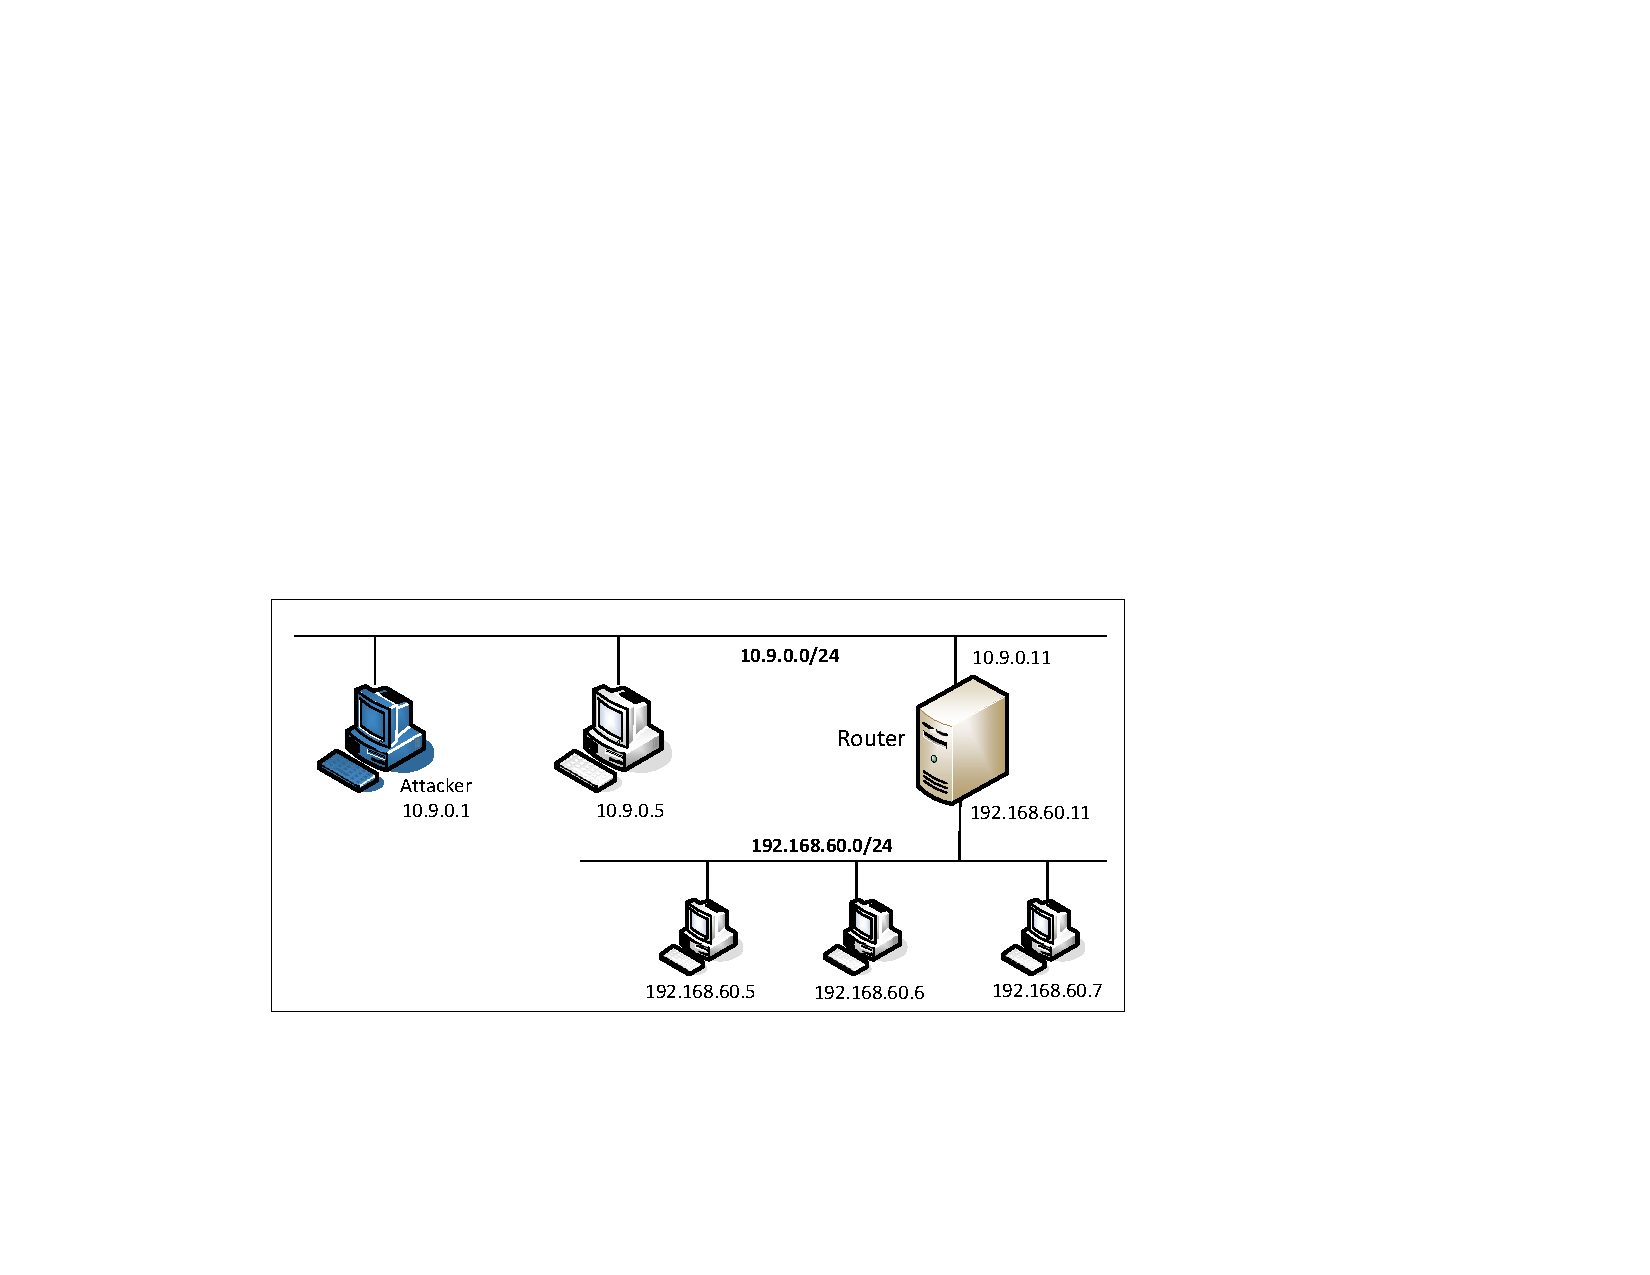
\includegraphics[width=0.8\textwidth]{./Figs/TwoLANs.pdf}
%\end{center}
%\caption{Setup del Laboratorio}
%\label{fig:labsetup}
%\end{figure}


% -------------------------------------------
% SUBSECTION
% -------------------------------------------
\subsection{Setup del Contenedor y sus Comandos}
%%%%%%%%%%%%%%%%%%%%%%%%%%%%%%%%%%%%%%%%%%%%
Para empezar a preparar el contenedor, deberá descargarse el archivo \texttt{Labsetup.zip} ubicado en el laboratorio correspondiente dentro del sitio web oficial y copiarlo dentro de la Máquina Virtual prevista por SEED. Una vez descargado deberá descomprimirlo y entrar dentro del directorio \texttt{Labsetup} donde encontrará el archivo \texttt{docker-compose.yml} que servirá para setear el entorno de laboratorio. Para una información más detallada sobre el archivo \texttt{Dockerfile} y otros archivos relacionados, puede encontrarla dentro del Manual de Usuario del laboratorio en uso, en el sitio web oficial de SEED.

Si esta es su primera experiencia haciendo el setup del laboratorio usando contenedores es recomendable que lea el manual anteriormente mencionado.

A continuación, se muestran los comandos más usados en Docker y Compose.
Debido a que estos comandos serán usados con mucha frecuencia, hemos creados un conjunto de alias para los mismos, ubicados en del archivo \texttt{.bashrc} dentro de la Máquina Virtual provista por SEED (Ubuntu 20.04)

\begin{lstlisting}
$ docker-compose build  # Build the container image
$ docker-compose up     # Start the container
$ docker-compose down   # Shut down the container

// Aliases for the Compose commands above
$ dcbuild       # Alias for: docker-compose build
$ dcup          # Alias for: docker-compose up
$ dcdown        # Alias for: docker-compose down
\end{lstlisting}


Dado que todos los contenedores estarán corriendo en un segundo plano. Necesitamos correr comandos para interactuar con los mismos, una de las operaciones fundamentales es obtener una shell en el contenedor. 
Para este propósito usaremos \texttt{"docker ps"} para encontrar el ID del contenedor deseado y ingresaremos \texttt{"docker exec"} para correr una shell en ese contenedor.
Hemos creado un alias para ello dentro del archivo \texttt{.bashrc}

\begin{lstlisting}
$ dockps        // Alias for: docker ps --format "{{.ID}}  {{.Names}}" 
$ docksh <id>   // Alias for: docker exec -it <id> /bin/bash

// The following example shows how to get a shell inside hostC
$ dockps
b1004832e275  hostA-10.9.0.5
0af4ea7a3e2e  hostB-10.9.0.6
9652715c8e0a  hostC-10.9.0.7

$ docksh 96
root@9652715c8e0a:/#  

// Note: If a docker command requires a container ID, you do not need to 
//       type the entire ID string. Typing the first few characters will 
//       be sufficient, as long as they are unique among all the containers. 
\end{lstlisting}

En caso de problemas configurando el entorno, por favor consulte la sección ``Common Problems'' en el manual ofrecido por SEED. 


%%%%%%%%%%%%%%%%%%%%%%%%%%%%%%%%%%%%%%%%%%%%




% -------------------------------------------
% SUBSECTION
% -------------------------------------------
% It does not seem to be necessary for this lab, 
% so let's comment this out.
%\subsection{Detach the VM from \texttt{192.168.60.0/24} Network} 
%%%%%%%%%%%%%%%%%%%%%%%%%%%%%%%%%%%%%%%%%%%%
%
%\paragraph{Removing the Host VM from \texttt{192.168.60.0/24} network.}

Cuando Docker crea una red, este automáticamente hace un attach de la máquina host (es decir la Máquina Virtual) hacía la red. En este caso, la máquina host es atachada en ambas redes, por lo que tendrá la IPs \texttt{10.9.0.1} y
\texttt{192.168.60.1}.
Estoo puede crear comportamientos no deseados, procederemos a remover este tipo de configuración.

En nuestro setup, solamente queremos que la Máquina Virtual este conectada a la red \texttt{10.9.0.0/24}.
Para esto necesitamos detachar la Máquina Virtual del resto de las redes, pero no podemos desactivar la interfaz de red dado que esto afectará a todos los contenedores que se encuentren en esa red.
La solución es borrar la dirección IP de la interfaz y reconfigurar el ruteo de la misma.


\begin{lstlisting}
// Get the name of the interface 
$ ip addr

// Remove the IP address from the interface
$ sudo ip addr flush <interface-name>

// Use 10.9.0.11 as the router to access 192.168.60.0/24
$ sudo ip route add 192.168.60.0/24 via 10.9.0.11
\end{lstlisting}


%%%%%%%%%%%%%%%%%%%%%%%%%%%%%%%%%%%%%%%%%%%%


% *******************************************
% SECTION
% ******************************************* 
\section{Tarea 1: Implementando un Firewall Simple} 

En esta tarea, implementaremos un firewall simple para filtrar paquetes, el mismo inspeccionará los paquetes que entren y salgan y será reforzado por las políticas establecidas por el administrador. Dado que el procesamiento de paquetes se hace dentro del kernel, el filtrado también debe ser hecho dentro del mismo. Aunque pareciera que dicho firewall requiere modificar el kernel de \linux. En el pasado se hacía modificando y recompilando el kernel. Hoy por hoy, los sistemas operativos \linux modernos nos proveen nuevos mecanismos para facilitarnos la manipulación de los paquetes sin la necesidad de recompilar la imagen del kernel. Esos dos mecanismos son \textit{Loadable Kernel Module} (\texttt{LKM}) y \texttt{Netfilter}.



\paragraph{Notas sobre los contenedores.}
Dado que todos los contenedores comparten el mismo kernel, los módulos del kernel son globales.
Además si seteamos un modelo de kernel para un contenedor, este afectará al resto de los contenedores y al host. Por esta razón, no importa donde ponga el módulo del kernel. En este laboratorio, lo haremos desde la máquina virtual host.

Otra cosa a tener en cuenta que es la dirección IP de los contenedores son virtuales.
Los paquetes que irán a esas direcciones IPs virtuales pueden que no recorran todas el mismo camino como se describe en la documentación de Netfilter.
Aunque para esta tarea, lo haremos lo menos confuso posible y trataremos de evitar esas direcciones virtuales.
Haremos la mayoría de las tareas en la máquina virtual host. Los contenedores se utilizarán para otras tareas.

% -------------------------------------------
% SUBSECTION
% ------------------------------------------- 
\subsection{Tarea 1.A: Implementar un Módulo de Kernel Simple}

{\tt LKM} nos permite agregar un nuevo módulo en el kernel en tiempo de ejecución.
Este módulo nos permite extender funcionalidades del kernel, sin recompilarlo o reiniciar la máquina.
El filtrado de paquetes de un firewall puede ser implementado como un LKM.
En esta tarea, nos familiarizaremos con LKM.

El siguiente código es un LKM. Este muestra \texttt{"Hello World!"} cuando este módulo es cargado; cuando el módulo se borra del kernel, este muestra \texttt{"Bye-bye World!"}.
Los mensajes no son impresos en pantalla; se muestran dentro del archivo \texttt{/var/log/syslog}. Puede usar el comando \texttt{"dmesg"} para visualizar los mensajes.


\begin{lstlisting}[language=C, caption=\texttt{hello.c} (included in the lab setup files)]
#include <linux/module.h>
#include <linux/kernel.h>

int initialization(void)
{
    printk(KERN_INFO "Hello World!\n");
    return 0;
}

void cleanup(void)
{
    printk(KERN_INFO "Bye-bye World!.\n");
}

module_init(initialization);
module_exit(cleanup);
\end{lstlisting}

Necesitamos crear el {\tt Makefile}, que incluye el siguiente contenido (este archivo esta incluído dentro los archivos de setup del laboratorio).
Sólo escriba {\tt make}, y el programa será compilado como un LKM (si ud. copia y pega lo siguiente dentro del archivo \texttt{Makefile}, asegúrese de reemplazar los espacios por tabs antes de ejecutar el comando \texttt{make}).


\begin{lstlisting}
obj-m += hello.o

all:
        make -C /lib/modules/$(shell uname -r)/build M=$(PWD) modules

clean:
        make -C /lib/modules/$(shell uname -r)/build M=$(PWD) clean
\end{lstlisting}

El módulo del kernel generado es \texttt{hello.ko}. 
Puede usar el siguiente comando para cargar el módulo, listar todos los módulos y borrar el módulo.
También puede usar \texttt{"modinfo hello.ko"} para ver información sobre un módulo específico del kernel.

\begin{lstlisting}
$ sudo insmod hello.ko     (inserting a module)
$ lsmod | grep hello       (list modules)
$ sudo rmmod hello         (remove the module)
$ dmesg                    (check the messages)
\end{lstlisting}


\paragraph{Tarea.} Por favor compile este LKM en su Máquina Virtual y ejecútelo. Para esta tarea, no usaremos contenedores. Por favor muestre sus resultados en el informe del laboratorio.


% -------------------------------------------
% SUBSECTION
% ------------------------------------------- 
\subsection{Tarea 1.B: Implementar un Firewall Simple usando \texttt{Netfilter}}  

En esta tarea, escribiremos nuestro programa para filtrar paquetes como un LKM y lo insertaremos dentro de la cadena de procesamientos de paquetes en el kernel. Esto no era fácil de hacer en el pasado, antes que \netfilter fuera introducido dentro de \linux.

{\tt Netfilter} está diseñado para facilitar la manipulación de los paquetes por usuarios autorizados. Logra su objetivo implementando una serie de hooks en el kernel de \linux. Estos hooks son intertados en varios lugares, incluyendo en los caminos de entrada y salida de paquetes.
Si queremos manipular los paquetes entrantes, solamente necesitamos conectar nuestro programa (dentro de un LKM) al hook que corresponde. Una vez que llega un paquete nuestro programa será invocado. Nuestro programa puede decidir si ese paquete debería de ser bloqueado o no; mas aún, podemos modificar los paquetes en el programa.

En esta tarea, ud. necesita usar LKM y {\tt Netfilter} para implementar un módulo de filtrado de paquetes. Este módulo obtendrá las políticas del firewall desde una estructura de datos y usará esta política para decidir si los paquetes deben de ser bloqueados o no.
Quisieramos que los estudiantes se enfoquen en la parte del filtrado, ya que es el núcleo de los firewalls, a los estudiantes se les permite hardcodear las políticas del firewall en el programa. Para una guía más detallada en como usar \texttt{Netfilter} puede consultar el Capítulo 17 del libro de SEED. 
En este documento también proveeremos guías.


\paragraph{Hookeando en \texttt{Netfilter}.} 

Usar \netfilter es relativamente sencillo. Todo lo que necesitamos hacer es hookear nuestras funciones (en el módulo kernel) a los hooks correspondientes de \netfilter. Aquí mostramos un ejemplo (el código está dentro de \path{Labsetup/packet_filter}), pero puede que no sea exactamente el mismo que se muestra en este ejemplo.
La estructura del código sigue la estructura del módulo del kernel implementado anteriormente. Cuando el módulo del kernel es agregado al kernel linux, la función \texttt{registerFilter()} que se encuentra en el código será invocada. Dentro de esta función, registramos dos hooks en \netfilter.

Para registrar un hook, necesita preparar una estructura de datos para el hook y setear todos los parámetros que son necesarios, el más importante es el nombre de la función (Línea \ding{202}) y el número de hook (Línea \ding{203}).
El número de hook es uno de los 5 hooks en \netfilter y la función especificada será invocada cuando un paquete llegue a este hook. En este ejemplo, cuando un paquete llega al hook \texttt{LOCAL\_IN}, la función \texttt{printInfo()} será invocada (esta función será desarrollada más adelante). Una vez que la estructura de datos para hook es preparada, atachamos el hook a \netfilter (Línea \ding{204})


\begin{lstlisting}[language=C, caption={Register hook functions to \netfilter}]
static struct nf_hook_ops hook1, hook2;

int registerFilter(void) {
   printk(KERN_INFO "Registering filters.\n");
   
   // Hook 1
   hook1.hook = printInfo;                    (*@\ding{202}@*)
   hook1.hooknum = NF_INET_LOCAL_IN;          (*@\ding{203}@*)
   hook1.pf = PF_INET;
   hook1.priority = NF_IP_PRI_FIRST;
   nf_register_net_hook(&init_net, &hook1);   (*@\ding{204}@*)

   // Hook 2
   hook2.hook = blockUDP;
   hook2.hooknum = NF_INET_POST_ROUTING;
   hook2.pf = PF_INET;
   hook2.priority = NF_IP_PRI_FIRST;
   nf_register_net_hook(&init_net, &hook2);

   return 0;
}

void removeFilter(void) {
   printk(KERN_INFO "The filters are being removed.\n");
   nf_unregister_net_hook(&init_net, &hook1);
   nf_unregister_net_hook(&init_net, &hook2);
}

module_init(registerFilter);
module_exit(removeFilter);
\end{lstlisting}

\paragraph{Nota para la Máquina Virtual de Ubuntu 20.04:}
El código en el libro de SEED fue desarrollado en Ubuntu 16.04. Este código necesita ser modificado levemente para que funcione en Ubuntu 20.04, el cambio está en la registración del hook y en la API de desregistración. A continuación puede observar las diferencias:


\begin{lstlisting}[language=C]
// Hook registration:
  nf_register_hook(&nfho);                  // For Ubuntu 16.04 VM
  nf_register_net_hook(&init_net, &nfho);   // For Ubuntu 20.04 VM

// Hook unregistration:
  nf_unregister_hook(&nfho);                // For Ubuntu 16.04 VM
  nf_unregister_net_hook(&init_net, &nfho); // For Ubuntu 20.04 VM
\end{lstlisting}
 

\paragraph{Funciones Hook.} A continuación daremos un ejemplo de una función hook. Este hook mostrará la información del paquete.
Cuando \netfilter invoca una función hook, le pasa tres argumentos a esta función, incluyendo un puntero al paquete actual (\texttt{skb}). 
En el siguiente código, la Línea \ding{202} muestra como obtener el número de hook del argumento \texttt{state}.
En la Línea \ding{203}, usamos la función \texttt{ip\_hdr()} para obtener el puntero para el encabezado IP, y entonces usamos el especificador de formato de cadena \texttt{\%pI4} para mostrar la dirección IP de origen y destino en la Línea \ding{204}.

\begin{lstlisting}[language=C, caption={An example of hook function}]
unsigned int printInfo(void *priv, struct sk_buff *skb,   
                       const struct nf_hook_state *state)
{
   struct iphdr *iph;
   char *hook;

   switch (state->hook){          (*@\ding{202}@*)
     case NF_INET_LOCAL_IN: 
          printk("*** LOCAL_IN"); break;
     .. (code omitted) ...
   }

   iph = ip_hdr(skb);             (*@\ding{203}@*)           
   printk("    %pI4  --> %pI4\n", &(iph->saddr), &(iph->daddr)); (*@\ding{204}@*)
   return NF_ACCEPT;
}
\end{lstlisting}

Si necesita obtener los encabezados para otros protocolos, puede usar la siguiente funciones que se encuentran definidas en varios archivos de encabezado. La definición de la estructura de esos encabezados pueden ser encontradas dentro del directorio \path{/lib/modules/5.4.0-54-generic/build/include/uapi/linux}, donde el número de versión del directorio es el resultado de \texttt{"uname -r"}, por lo que puede variar de acuerdo a la versión de kernel que tenga instalada.

\begin{lstlisting}[language=C]
struct iphdr   *iph   = ip_hdr(skb)    // (need to include <linux/ip.h>) 
struct tcphdr  *tcph  = tcp_hdr(skb)   // (need to include <linux/tcp.h>) 
struct udphdr  *udph  = udp_hdr(skb)   // (need to include <linux/udp.h>) 
struct icmphdr *icmph = icmp_hdr(skb)  // (need to include <linux/icmp.h>) 
\end{lstlisting}
 

\paragraph{Bloqueando paquetes.} 
También ofrecemos un ejemplo de una función hook para mostrar como bloquear un paquete si este cumple con una condición específica. El siguiente ejemplo bloquea paquetes UDP si su dirección IP de destino es \texttt{8.8.8.8} y el puerto de destino es \texttt{53}. Esto significa que bloqueará las consultas DNS al nameserver \texttt{8.8.8.8}. 

\begin{lstlisting}[language=C, caption={Code example: blocking UDP}]
unsigned int blockUDP(void *priv, struct sk_buff *skb,
                 const struct nf_hook_state *state)
{
   struct iphdr *iph;
   struct udphdr *udph;
   u32  ip_addr;
   char ip[16] = "8.8.8.8";

   // Convert the IPv4 address from dotted decimal to a 32-bit number
   in4_pton(ip, -1, (u8 *)&ip_addr, '\0', NULL);                  (*@\ding{202}@*)
   
   iph = ip_hdr(skb);
   if (iph->protocol == IPPROTO_UDP) {
       udph = udp_hdr(skb);                                         
       if (iph->daddr == ip_addr && ntohs(udph->dest) == 53){     (*@\ding{203}@*)
            printk(KERN_DEBUG "****Dropping %pI4 (UDP), port %d\n", 
                              &(iph->daddr), port);                 
            return NF_DROP;                                       (*@\ding{204}@*)
        }
   }
   return NF_ACCEPT;                                              (*@\ding{205}@*)
}
\end{lstlisting}

En el código anterior, la Línea \ding{202} muestra como convertir dentro del kernel, una dirección IP en formato decimal con punto (es decir una cadena, como sería \texttt{1.2.3.4}) en un binario de 32-bits (\texttt{0x01020304}), por lo que puede ser comparado con el número binario que está guardado dentro de los paquetes.
La Línea \ding{203} compara la dirección IP de destino y el número de puerto con los valores de nuestra regla. Si estos valores coinciden con los de la regla,  \texttt{NF\_DROP} será retornado a \netfilter que se encargará de dropear el paquete. En caso contrario, \texttt{NF\_ACCEPT} será retornado y \netfilter dejará que el paquete continue su viaje (\texttt{NF\_ACCEPT} quiere decir que el paquete es aceptado por esta función hook; pero aún así puede ser dropeado por otra función hook).

\paragraph{Tareas.} El código completo de muestra se llama \texttt{seedFilter.c} y está incluído en los archivos del laboratorio (dentro del directorio \path{Files/packet_filter}). Por favor realize las siguientes tareas (hágalas por separado).

\begin{enumerate}
	
\item Compile el código de ejemplo usando el archivo \texttt{Makefile} que se encuentra dentro de los archivos del laboratorio.
	Cargue este código dentro del kernel y demuestre que el firewall está trabajando como se espera. Puede usar el siguiente comando para generar paquetes UDP hacia \texttt{8.8.8.8}, que son los servidores DNS de Google. Si su firewall funciona, sus peticiones serán bloqueadas; de otra forma, ud. obtendrá una respuesta.

\begin{lstlisting}
dig @8.8.8.8 www.example.com 
\end{lstlisting}
 
\item Hookee la función \texttt{printInfo} en todos los hooks de \netfilter. Aquí están las macros de los números de hooks. 
Usando los resultados de su experimento, explique en que condiciones la función de cada uno de los hooks es invocada.

\begin{lstlisting}
NF_INET_PRE_ROUTING 
NF_INET_LOCAL_IN        
NF_INET_FORWARD 
NF_INET_LOCAL_OUT 
NF_INET_POST_ROUTING    
\end{lstlisting}


\item Implemente dos hooks más para lograr lo siguiente:
(1) prevenir que otras máquinas hagan ping a la Máquina virtual y (2) prevenir que otras máquinas puedan hacer telnet a la máquina virtual.
Por favor implemente dos funciones hooks diferentes, pero registrelas en el mismo hook \netfilter. Ud. debe de decidir que hook usar.
El puerto default de telnet es \texttt{23}. Para probarlo, puede iniciar los contenedores, ir a \texttt{10.9.0.5} y ejecutar los siguientes comandos (\texttt{10.9.0.1} es la dirección IP asignada a la Máquina Virtual; para hacer las cosas más simples, puede hardcodear esta IP en las reglas del firewall):

 
\begin{lstlisting}
ping 10.9.0.1
telnet 10.9.0.1
\end{lstlisting}
     
\end{enumerate}
 

\paragraph{Nota importante:} Debido a que hemos hecho cambios en el kernel, hay altas chances que el kernel pueda crashear. Asegúrese de hacer un backup de sus archivos con frecuencia. Una de las razones más comunes por la cual el sistema puede crashear es si ud. olvida de desregistrar los hooks. Cuando un módulo es borrado, esos hooks serán llamados pero el módulo no estará presente en el kernel. Eso causará que el sistema crashee.
Para evitar esto, asegúrese que por cada hook que ud. agrega en su módulo, agregue una línea en \texttt{removeFilter} para desregistrarlo, por lo que cuando el módulo es borrado, esos hooks sean removidos también.


% *******************************************
% SECTION
% ******************************************* 
\section{Tarea 2: Experimentando Reglas en un Firewall Stateless}

En las tareas anteriores, tuvimos la chance de construir un firewall simple usando \netfilter. Actualmente, \linux tiene un firewall integrado basado en \netfilter. Este firewall se llama \iptables. Técnicamente la parte del kernel que implementa el firewall se llama  \texttt{Xtables}, mientras que \iptables es un programa en user-space para configurar el firewall. Sin embargo \iptables es usado a menudo para referirse a la implementación a nivel kernel y a nivel usuario.



% -------------------------------------------
% SUBSECTION
% ------------------------------------------- 
\subsection{Background de \iptables}

En esta tarea, usaremos \iptables para hacer el setup de un firewall.
El firewall \iptables está diseñado no solamente para filtrar paquetes, sino también para modificarlos. Para manejar los diferentes propósitos de las reglas del firewall, \iptables organiza todas sus reglas en una estructura jerárquica: table, chain y rules (tablas, cadenas y reglas).
Existen varias tablas, cada una especifica el propósito principal de las reglas como se muestra en la Tabla \ref{firewall:table:iptables}.
Por ejemplo, las reglas para el filtrado de paquetes deberían de ser ubicadas en la tabla \texttt{filter}, mientras que las reglas para hacer cambios en lo paquetes deberían de ser ubicadas en las tablas \texttt{nat} o \texttt{mangle}.

Cada tabla contiene varias cadenas, cada una corresponde a un hook de \netfilter. Básicamente, cada cadena indica donde se refuerzan sus reglas. Por ejemplo, las reglas en la cadena \texttt{FORWARD} son reforzadas en el hook \texttt{NF\_INET\_FORWARD} y las reglas en la cadena \texttt{INPUT} son reforzadas en el hook \texttt{NF\_INET\_LOCAL\_IN}.

Cada cadena contiene un conjunto de reglas de firewall que serán reforzadas.
Cuando configuramos firewalls, agregamos reglas en esas cadenas.
Por ejemplo, si quisieramos bloquear todo el tráfico \telnet entrante, agregaríamos una regla en la cadena \texttt{INPUT} de la tabla \texttt{filter}. Si quisieramos redireccionar todo el tráfico \telnet hacia un puerto  en un host diferente, básicamente estaríamos haciendo port forwarding, podemos agregar una regla en la cadena \texttt{INPUT} de la tabla \texttt{mangle}, si necesitamos hacer cambios en los paquetes.


\begin{table}[htb]
        \centering
%       \renewcommand{\arraystretch}{1.2}
        \caption{\iptables Tables and Chains}
        \label{firewall:table:iptables}
        \centering

        \begin{tabular}{|l|l|l|}
                \hline
                \bfseries Table & \bfseries Chain & \bfseries Functionality \\
                \hline\hline
                filter          &    \texttt{INPUT}      & Packet filtering \\
                                &    \texttt{FORWARD}    & \\
                                &    \texttt{OUTPUT}      & \\
                \hline
                nat             &   \texttt{PREROUTING}    & Modifying source or destination \\
                                &   \texttt{INPUT}      & network addresses \\
                                &   \texttt{OUTPUT}      & \\
                                &   \texttt{POSTROUTING}   & \\
                \hline
                mangle          &   \texttt{PREROUTING}    & Packet content modification \\
                                &   \texttt{INPUT}      & \\
                                &   \texttt{FORWARD}     & \\
                                &   \texttt{OUTPUT}      & \\
                                &   \texttt{POSTROUTING}   & \\
                \hline
        \end{tabular}
\end{table}


% -------------------------------------------
% SUBSECTION
% ------------------------------------------- 
\subsection{Usando \iptables}

Para agregar reglas en las cadenas de cada una de las tablas, usamos el comando \iptables, este comando es bastante poderoso.
Los estudiantes pueden ver el manual de \iptables tipeando \texttt{"man iptables"} o buscando tutoriales en la red.
Lo que hace de \iptables complicado es la cantidad de argumentos de consola que necesitamos aplicar cuando se usa este programa. Sin embargo, si entendemos la estructura de estos argumentos, descubriremos que \iptables no es tan complicado.

En una situación típica, usamos el comando \iptables para agregar o borrar una regla de alguna de las cadenas en algunas de las tablas, por lo que necesitamos especificar el nombre de la tabla (por defecto es \texttt{filter}), un nombre de cadena y una operación en esa cadena. Después de eso, especificamos la regla, que es básicamente un patrón que coincidirá o no con cada uno de los paquetes que pasan por el firewall. Si coincide con la regla, una acción será ejecutada sobre este paquete.
La estructura general de un comando de \iptables es ilustrada a continuación:

\begin{lstlisting}
iptables -t <table> -<operation> <chain>  <rule>   -j <target>
         ---------- --------------------  -------  -----------
            Table          Chain           Rule      Action
\end{lstlisting}

La parte más complicada del comando \iptables es la regla.
Más adelante profundizaremos sobre este asunto cuando usemos reglas específicas. A continuación se listan algunos comandos básicos de uso común:


\begin{lstlisting}
// List all the rules in a table (without line number)
iptables -t nat -L -n

// List all the rules in a table (with line number)
iptables -t filter -L -n --line-numbers


// Delete rule No. 2 in the INPUT chain of the filter table 
iptables -t filter -D INPUT 2

// Drop all the incoming packets that satisfy the <rule>
iptables -t filter -A INPUT <rule>  -j DROP
\end{lstlisting}


\paragraph{Nota.} Docker descansa en \iptables para manejar la red que crea, este agrega muchas reglas en la tabla \texttt{nat}.
Cuando manipulamos las reglas de \iptables, debemos de ser cuidadosos en no remover las reglas de Docker. Por ejemplo, sería algo peligroso ejecutar el comando \texttt{"iptables -t nat -F"}, porque borraría todas las reglas en la tabla \texttt{nat}, incluídas muchas reglas de Docker. Eso causará conflictos en los contenedores de Docker. Haciendo esto para la tabla \texttt{filter} está bien, porque Docker no toca esta tabla.


% -------------------------------------------
% SUBSECTION
% -------------------------------------------
\subsection{Tarea 2.A: Protegiendo el Router} 

En esta tarea, crearemos reglas en el firewall para prevenir el acceso de máquinas externas a la máquina router, excepto por el ping.
Por favor ejecute el siguiente comando \iptables en el contenedor router y trate de accederlo desde \texttt{10.9.0.5}. (1) ¿Puede hacer ping al router? (2) ¿Puede hacer telnet al router? (el servicio de telnet se encuentra corriendo en todos los contenedores; se ha creado una cuenta llamada \texttt{seed} y su password es \texttt{dees}).
Por favor reporte su observación y explique el propósito de cada regla.


\begin{lstlisting}
iptables -A INPUT  -p icmp --icmp-type echo-request -j ACCEPT
iptables -A OUTPUT -p icmp --icmp-type echo-reply   -j ACCEPT
iptables -P OUTPUT DROP     (*@\pointleft{Set default rule for OUTPUT}@*)
iptables -P INPUT  DROP     (*@\pointleft{Set default rule for INPUT}@*)
\end{lstlisting}
 

\paragraph{Limpieza.} 
Antes de movernos a la próximo tarea, por favor restaure la tabla \texttt{filter} a su estado original ejecutando los siguientes comandos:

\begin{lstlisting}
iptables -F
iptables -P OUTPUT ACCEPT
iptables -P INPUT  ACCEPT
\end{lstlisting}

Otra forma de restaurar los estados de todas las tablas es reiniciando el contenedor. Puede hacerlo usando el siguiente comando (necesita encontrar el ID del contenedor primero):

\begin{lstlisting}
$ docker restart <Container ID>
\end{lstlisting}
 


% -------------------------------------------
% SUBSECTION
% -------------------------------------------
\subsection{Tarea 2.B: Protegiendo la Red Interna} 

En esta tarea, crearemos reglas en el firewall del router para proteger la red interna \texttt{192.168.60.0/24}. Para esto necesitaremos usar la cadena FORWARD.

La dirección de los paquetes en las cadenas INPUT y OUPUT son claras:
los paquetes entran por INPUT y salen por OUTPUT.
Esto no es así para la cadena FORWARD, esta es bidireccional: los paquetes que se dirigen a la red interna o salen a la red externa pasan siempre por esta cadena. Para especificar la dirección, podemos agregar la opción de interfaz usando \texttt{"-i xyz"} (viene desde la interfaz \texttt{xyz}) y/o \texttt{"-o xyz"} (sale desde la interfaz \texttt{xyz}). Las interfaces para la red interna y externa son diferentes.
Puede encontrar los nombres de las interfaces usando el comando \texttt{"ip addr"}.

En esta tarea, queremos implementar un firewall para proteger la red interna. Más específicamente, necesitamos reforzar las siguientes restricciones en el tráfico ICMP:


\begin{enumerate}[noitemsep]
  \item	Los hosts externos no pueden hacer ping a los hosts internos.
  \item	Los hosts externos pueden hacer ping al router.
  \item	Los hosts internos pueden hacer ping a los hosts externos.
  \item	El resto de los paquetes entre las redes interna y externa deben de ser bloqueados.
\end{enumerate}

Necesitará usar la opción \texttt{"-p icmp"} para especificar la condición relacionada al protocolo ICMP. Puede ejecutar \texttt{"iptables -p icmp -h"} para ver todas las condiciones ICMP. El siguiente ejemplo dropea una petición echo ICMP.


\begin{lstlisting}
iptables -A FORWARD -p icmp --icmp-type echo-request -j DROP
\end{lstlisting}

En su informe del laboratio, por favor incluya sus reglas y las capturas de pantalla para demostrar que su firewall funciona como es esperado.
Cuando termine con esta tarea, por favor recuerde limpiar las tablas o reiniciar el contenedor, antes de moverse a la siguiente tarea.

% -------------------------------------------
% SUBSECTION
% -------------------------------------------
\subsection{Tarea 2.C: Protegiendo los Servicios Internos}

En esta tarea, queremos proteger los servidores TCP dentro de la red interna  (\texttt{192.168.60.0/24}). 
Más específicamente, quisieramos lograr los siguientes objetivos.

\begin{enumerate}[noitemsep]
	
  \item Todos los hosts internos corren un servidor telnet (escuchando en el puerto \texttt{23}).
  Los hosts externos sólo pueden acceder al servidor telnet en \texttt{192.168.60.5}, y no al resto de los hosts de la red interna.
  
  \item Los hosts externos no pueden acceder a los servidores internos.

  \item Los hosts internos pueden acceder a todos los servidores internos.

  \item Los hosts internos no pueden acceder a los servidores externos.
  
  \item En esta tarea, no se permite el mecanismo del trackeo de conexión (connection tracking). Será usado en una tarea posterior.
\end{enumerate}

Necesitará usar la opción  \texttt{"-p tcp"} para especificar la condición que debe de coincidir para el protocolo TCP. Puede ejecutar \texttt{"iptables -p tcp -h"} para encontrar todas las condiciones de matcheo para TCP. El siguiente ejemplo deja  que los paquetes TCP pque vienen de la interfaz  \texttt{eth0} si su puerto origen es \texttt{5000}, pasen por el firewall.


\begin{lstlisting}
iptables -A FORWARD -i eth0 -p tcp --sport 5000  -j ACCEPT
\end{lstlisting}

Cuando termine con esta tarea, recuerde limpiar las tablas o reiniciar el contenedor antes de proceder a la siguiente tarea.




% *******************************************
% SECTION
% ******************************************* 
\section{Tarea 3: Trackeo de Conexión (connection tracking) y Firewall Stateful}

En la tarea anterior, hemos trabajado con firewalls stateless, que inspeccionan cada paquete de forma independiente. Sin embargo, los paquetes generalmente no son independiente; ellos pueden ser parte de una conexión TCP o pueden ser paquetes ICMP ejecutados por otros paquetes. Tratarlos como independientes no toma en consideración el contexto de los paquetes, y puede desembocar en reglas poco precisas, inseguras o complejas.
Poir ejemplo, si quisieramos dejar que entren paquetes TCP en nuestra red sólo si hubo una primera conexión, no lo podemos hacer de forma fácil usando un filtrado de paquetes stateless, porque cuando el firewall examine cada paquete TCP de forma individual, no tendrá idea si el paquete pertenece a una conexión existente o no, al menos que el firewall mantenga alguna información sobre el estado de cada conexión.
Si eso se cumple, estamos en presencia de un firewall stateful.

% -------------------------------------------
% SUBSECTION
% ------------------------------------------- 
\subsection{Tarea 3.A: Experimentado con el Trackeo de Conexiones} 

Para dar soporte a un firewall stateful, necesitamos poder trackear las conexiones.
Esto se logra con el mecanismo \texttt{conntrack} dentro del kernel.
En esta tarea, haremos experimentos relacionados con este módulo y nos familiarizaremos con el mecanismo del trackeo de conexiones o connection tracking.
En nuestro experimento, chequeremos la información del trackeo de conexión en el contenedor del router. Esto puede hacerse usando el siguiente comando:

\begin{lstlisting}
# conntrack -L
\end{lstlisting}

El objetivo de la tarea es usar una serie de experimentos para ayudar a los estudiantes a entender el concepto de conexión en este mecanismo de tracking, especialmente para los protocolos ICMP y UDP, porque a diferencia de TCP, ellos no tienen conexiones.
Por favor realize los siguientes experimentos. Por cada experimento, por favor describa su observación junto con su explicación.

\begin{itemize}
\item Experimento ICMP: Ejecute el siguiente comando y observe la información del trackeo de conexión en el router. Describa su observación. ¿Cuanto tiempo se mantiene el estado de la conexión ICMP?

\begin{lstlisting}
// On 10.9.0.5, send out ICMP packets
# ping 192.168.60.5
\end{lstlisting}

\item Experimento UDP:Ejecute el siguiente comando y observe la información del trackeo de conexión en el router. Describa su observación. ¿Cuanto tiempo se mantiene el estado de la conexión UDP?


\begin{lstlisting}
// On 192.168.60.5, start a netcat UDP server
# nc -lu 9090

// On 10.9.0.5, send out UDP packets  
# nc -u 192.168.60.5 9090
<type something, then hit return>
\end{lstlisting}


\item Experimento TCP: Ejecute el siguiente comando y observe la información del trackeo de conexión en el router. Describa su observación. ¿Cuanto tiempo se mantiene el estado de la conexión TCP?

\begin{lstlisting}
// On 192.168.60.5, start a netcat TCP server
# nc -l 9090

// On 10.9.0.5, send out TCP packets 
# nc 192.168.60.5 9090
<type something, then hit return>
\end{lstlisting}

\end{itemize}
 


% -------------------------------------------
% SUBSECTION
% ------------------------------------------- 
\subsection{Tarea 3.B: Configurando un Firewall Stateful} 


Now we are ready to set up firewall rules based on connections. 
In the following example, 
the \texttt{"-m conntrack"} option indicates that we are using the \texttt{conntrack} module,
which is a very important module for \iptables; it tracks connections, and
\iptables replies on the tracking information to build stateful firewalls. 
The \texttt{--ctsate ESTABLISHED,RELATED} indicates that whether a packet
belongs to an \texttt{ESTABLISHED} or \texttt{RELATED} connection.
The rule allows TCP packets belonging to an existing connection to 
pass through. 

\begin{lstlisting}
iptables -A FORWARD -p tcp -m conntrack          \
         --ctstate ESTABLISHED,RELATED -j ACCEPT
\end{lstlisting}


The rule above does not cover the SYN packets, which do not belong to 
any established connection. Without it, we will not be able to 
create a connection in the first place. Therefore, we need to 
add a rule to accept incoming SYN packet: 

\begin{lstlisting}
iptables -A FORWARD -p tcp -i eth0 --dport 8080 --syn  \
         -m conntrack --ctstate NEW -j ACCEPT 
\end{lstlisting}

Finally, we will set the default policy on FORWARD to drop
everything. This way, if a packet is not accepted by the two
rules above, they will be dropped. 

\begin{lstlisting}
iptables -P FORWARD DROP
\end{lstlisting}


Please rewrite the firewall rules in Task 2.C, but this time,
\textbf{we will add a rule allowing internal hosts to visit any 
external server} (this was not allowed in Task 2.C). 
After you write the rules using the connection tracking mechanism, 
think about how to do it without using the connection tracking
mechanism (you do not need to actually implement them). 
Based on these two sets of rules, 
compare these two different approaches, and 
explain the advantage and disadvantage of each approach. 
When you are done with this task, remember to clear all the rules. 



% *******************************************
% SECTION
% ******************************************* 
\section{Tarea 4: Limitando el Tráfico de Red}

In addition to blocking packets, we can also 
limit the number of packets that can pass through the firewall. 
This can be done using the \texttt{limit} module of \iptables.
In this task, we will use this module to limit how many packets 
from \texttt{10.9.0.5} are allowed to get into the internal network. 
You can use \texttt{"iptables -m limit -h"} to see the manual.  

\begin{lstlisting}
$ iptables -m limit -h
limit match options:
--limit avg             max average match rate: default 3/hour
                        [Packets per second unless followed by
                        /sec /minute /hour /day postfixes]
--limit-burst number    number to match in a burst, default 5
\end{lstlisting}
 

Please run the following commands on router, and then
ping \texttt{192.168.60.5} from \texttt{10.9.0.5}.  
Describe your observation. 
Please conduct the experiment with and without the second rule, 
and then explain whether the second rule is needed or not, and why.

\begin{lstlisting}
iptables -A FORWARD -s 10.9.0.5 -m limit \
         --limit 10/minute --limit-burst 5 -j ACCEPT

iptables -A FORWARD -s 10.9.0.5 -j DROP
\end{lstlisting}



% *******************************************
% SECTION
% *******************************************
\section{Tarea 5: Balanceo de Carga}

The \iptables is very powerful. In addition to firewalls,
it has many other applications. We will not be able to 
cover all its applications in this lab, but we will experimenting
with one of the applications, load balancing. In this task,
we will use it to load balance three UDP servers running in the 
internal network. Let's first start the server
on each of the hosts: \texttt{192.168.60.5}, \texttt{192.168.60.6}, and 
\texttt{192.168.60.7} (the \texttt{-k} option indicates that 
the server can receive UDP datagrams from multiple hosts):

\begin{lstlisting}
nc -luk 8080
\end{lstlisting}

We can use the \texttt{statistic} module to achieve load balancing. 
You can type the following command to get its manual. You can 
see there are two modes: \texttt{random} and \texttt{nth}. 
We will conduct experiments using both of them.

\begin{lstlisting}
$ iptables -m statistic -h 
statistic match options:
 --mode mode         Match mode (random, nth)
 random mode:
[!] --probability p  Probability
 nth mode:
[!] --every n        Match every nth packet
 --packet p          Initial counter value (0 <= p <= n-1, default 0)
\end{lstlisting}
 

\paragraph{Usando el modo \texttt{nth} (round-robin).}
On the router container, we set the following rule, which applies 
to all the UDP packets going to port \texttt{8080}. 
The \texttt{nth} mode of the \texttt{statistic} module is used; 
it implements a round-robin load balancing policy: for every
three packets, pick the packet 0 (i.e., the first one), 
change its destination IP address and port number to 
\texttt{192.168.60.5}  and \texttt{8080}, respectively.  
The modified packets will continue on its journey.

\begin{lstlisting}
iptables -t nat -A PREROUTING -p udp --dport 8080      \
         -m statistic --mode nth --every 3 --packet 0  \
         -j DNAT --to-destination 192.168.60.5:8080
\end{lstlisting}

It should be noted that those packets that do not match
the rule will continue on their journeys; they will
not be modified or blocked. With this rule in place, 
if you send a UDP packet to the router's \texttt{8080} port,  
you will see that one out of three packets gets to 
\texttt{192.168.60.5}. 

\begin{lstlisting}
// On 10.9.0.5
echo hello | nc -u 10.9.0.11 8080
<hit Ctrl-C>
\end{lstlisting}
 

Please add more rules to the router container, 
so all the three internal hosts get the equal 
number of packets. 
Please provide some explanation for the rules. 


\paragraph{Usando el modo \texttt{random}.}
Let's use a different mode to achieve the load balancing. The following 
rule will select a matching packet with the probability \texttt{P}.  
You need to replace \texttt{P} with a probability number.

\begin{lstlisting}
iptables -t nat -A PREROUTING -p udp --dport 8080   \
         -m statistic --mode random --probability P \
         -j DNAT --to-destination 192.168.60.5:8080
\end{lstlisting}

Please use this mode to implement your load balancing 
rules, so each internal server get roughly the 
same amount of traffic (it may not be exactly the same, 
but should be close when the total number of packets is large). 
Please provide some explanation for the rules. 




% *******************************************
% SECTION
% ******************************************* 
\section{Informe del Laboratorio y Demostraciones}


%%%%%%%%%%%%%%%%%%%%%%%%%%%%%%%%%%%%%%%%

Debe enviar un informe de laboratorio detallado, con capturas de pantalla, para describir lo que ha hecho y lo que ha observado.
También debe proporcionar una explicación a las observaciones que sean interesantes o sorprendentes.
Enumere también los fragmentos de código más importantes seguidos de una explicación. No recibirán créditos aquellos fragmentos de códigos que no sean explicados.
%%%%%%%%%%%%%%%%%%%%%%%%%%%%%%%%%%%%%%%%

\section*{Agradecimientos}

Este documento ha sido traducido al Español por Facundo Fontana



\end{document}
%%%%%%%%%%%%%%%%%%%%%%%%%%%%%%%%%%%%%%%%%%%%%%%%%%%%%%%%
%%%%%%%%%%%%%%%%%%%%%%%%%%%%%%%%%%%%%%%%%%%%%%%%%%%%%%%%



